\documentclass[12pt]{article}

% --- Packages ---
\usepackage{amsmath, amsthm, amssymb}
\usepackage{graphicx}
\usepackage{geometry}
\usepackage{fancyhdr}
\usepackage{enumerate}
\usepackage{listings}
\usepackage{xcolor}
\usepackage{setspace}
\usepackage[utf8]{inputenc}
\usepackage[english]{babel}
\usepackage{framed}
\usepackage{caption}
\usepackage{booktabs}     % for \toprule etc.
\usepackage{siunitx}      % for \SI, units
\usepackage{array}
\usepackage{makecell}     % for multi-line table cells
\usepackage{tabularx}     % auto-wrapping column type X
\sisetup{detect-all, per-mode=symbol} % nicer units

% Keep hyperref LAST
\usepackage{hyperref}

% ragged-right X column that still allows \\ at row ends
\newcolumntype{Y}{>{\raggedright\arraybackslash}X}


% Page Layout
\geometry{
    textheight=9in,
    textwidth=5.5in,
    top=1in,
    headheight=12pt,
    headsep=25pt,
    footskip=30pt
}

\begin{document}
\begin{center}
    {\LARGE \textbf{Ultrasonic Sensor Timing Sequence}}\\[0.5em]
\end{center}
\begin{figure}[h!]
    \centering
    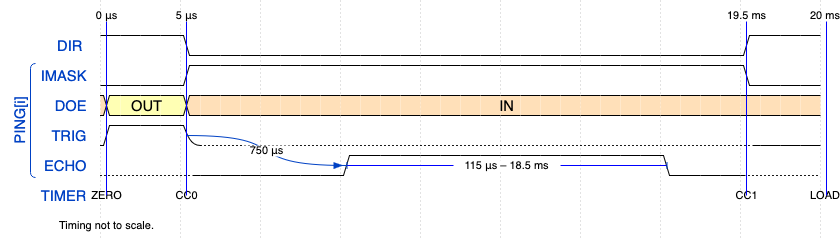
\includegraphics[width=0.95\linewidth]{ping_timing_diagram.png}
    \caption{\small PING))) Ultrasonic Sensor Timing Sequence (Single-Sensor Cycle).}
    \label{fig:ping_timing}
\end{figure}

\small

\noindent One full \SI{20}{ms} measurement cycle for a single \textbf{Parallax PING))) Ultrasonic Distance Sensor} via an \textbf{SN74LVC245A} bidirectional level shifter. The MCU issues a \SI{5}{\micro\second} trigger, then reconfigures the shared I/O to input to measure the echo pulse width (time-of-flight).

\begingroup\scriptsize
\vspace{4pt}
\begin{center}
\renewcommand{\arraystretch}{1.2}
\begin{tabularx}{\linewidth}{@{} l l Y @{}}
\toprule
\textbf{Signal} & \textbf{Name / Direction} & \textbf{Description} \\
\midrule
\textbf{DIR} & Buffer Direction &
\textit{SN74LVC245A} direction control.\newline
1 = MCU $\rightarrow$ Sensor (trigger phase).\newline
0 = Sensor $\rightarrow$ MCU (echo phase).\\[3pt]
\hline
\textbf{PING[$i$]} & Sensor GPIO (Group) &
Bidirectional MCU GPIO shared with ultrasonic sensor $i$.\newline
Logical group encompassing IMASK, DOE, TRIG, and ECHO signals.\newline
Manages the trigger, echo, and interrupt states for each sensor in the round-robin sequence.\\[3pt]
\hline
\textbf{IMASK} & Interrupt Mask &
Per-pin interrupt enable for the PING line.\newline
1 = Interrupt enabled (ECHO edge capture active).\newline
0 = Interrupt disabled (no capture events forwarded to NVIC).\\[3pt]
\hline
\textbf{DOE} & Data Output Enable &
MCU GPIO output-enable control for the PING line.\newline
Input: idle and echo phases (interrupts disabled during idle).\newline
Output: trigger phase.\\[3pt]
\hline
\textbf{TRIG} & Trigger Pulse &
\SI{5}{\micro\second} rising-edge pulse driven by MCU to initiate ultrasonic burst from the sensor.\\[3pt]
\hline
\textbf{ECHO} & Echo Pulse &
Return pulse width proportional to target distance.\newline
Minimum: \SI{115}{\micro\second}\newline
Maximum: \SI{18.5}{\milli\second}.\\[3pt]
\hline
\textbf{TIMER} & Capture / Compare &
Timer capture/compare reference points (ZERO, CC0, CC1, LOAD) aligned with echo pulse duration measurement.\\
\bottomrule
\end{tabularx}
\end{center}
\endgroup

\noindent\textbf{Notes.}
\begin{enumerate}
  \item Timer in edge-aligned up-count mode (LOAD = period limit).
  \item Preload GPIO output before asserting DOE to avoid transients.
  \item Round-robin across sensors with \SI{20}{ms} spacing to avoid ultrasonic crosstalk.
  \item SN74LVC245A provides \SI{5}{V} $\leftrightarrow$ \SI{3.3}{V} logic compatibility.
\end{enumerate}

\newpage
\begin{center}
    {\LARGE \textbf{Multi-Sensor Schedule Cycle}}\\[0.5em]
\end{center}

\begin{figure}[h!]
    \centering
    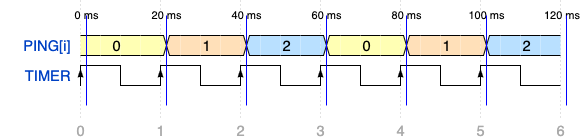
\includegraphics[width=0.95\linewidth]{ping_round_robin_diagram.png}
    \caption{\small Round-robin schedule for three ultrasonic sensors.}
    \label{fig:ping_round_robin}
\end{figure}

\small
\noindent The system operates three ultrasonic sensors in a round-robin sequence to prevent acoustic interference between transducers. Each sensor is allocated a dedicated \SI{20}{ms} time slot encompassing its trigger, echo measurement, and a brief guard interval before the next sensor’s cycle begins. This ensures that no two sensors emit ultrasonic bursts simultaneously.

\vspace{6pt}
\begin{center}
\renewcommand{\arraystretch}{1.15}
\begin{tabular}{ccc} % <-- centered columns
\toprule
\textbf{Slot} & \textbf{Time Window} & \textbf{Active Sensor} \\
\midrule
0 & $[\,\,\,\,\SI{0}{ms},\,\SI{20}{ms})$   & PING[0] \\
1 & $[\,\SI{20}{ms},\,\SI{40}{ms})$  & PING[1] \\
2 & $[\,\SI{40}{ms},\,\SI{60}{ms})$  & PING[2] \\
\bottomrule
\end{tabular}

\vspace{3pt}
\footnotesize
Cycle repeats every \SI{60}{ms}, yielding an update rate of \SI{16.7}{Hz} per sensor.
\end{center}
\vspace{6pt}
\noindent\textbf{Timing considerations.}
As shown in the single-sensor timing diagram, each measurement cycle consists of a short trigger, a fixed holdoff interval, and an echo pulse lasting up to approximately \SI{18.5}{ms}. Including these intervals yields a total cycle time of about \SI{19.2}{ms}, so a \SI{20}{ms} slot provides a small but sufficient margin to accommodate overhead and ensure all echoes have dissipated before the next sensor begins.\\
\\
\noindent\textbf{Notes.}
\begin{enumerate}
  \item Only one sensor is active per slot; the remaining sensors stay configured as inputs with their internal pull-downs enabled to prevent bus contention and maintain a defined low idle state. 
  \item The MCU cycles through sensors sequentially every \SI{20}{ms}.
  \item This schedule avoids cross-interference while maintaining a \SI{50}{Hz} global timing base.
  \item Additional sensors can be supported by proportionally extending the total cycle period.
\end{enumerate}
\end{document}

